\documentclass[%
  a4paper,%
  12pt,% <10pt, 9pt>
  style=screen, % TODO zum Drucken ausstellen
  %sender=bottom,
  oneside,
  %bcor = 0cm, % Keine Bindekorrektur 
  blue,% <orange, green, violet>
  %rgb, <cmyk>
  %mono,
  %extramargin,
  %marginleft, <marginright>
  ]{tubsartcl} 
 
% Packages:  
\usepackage[utf8x]{inputenc}
\usepackage[ngerman]{babel}
\usepackage[fixlanguage]{babelbib} % Deutsches Literaturverzeichnis
\usepackage[onehalfspacing]{setspace} % Zeilenabstand 1,5 zeilig
\usepackage[
    hidelinks, breaklinks % Farbige Boxen um Hyperlinks nicht anzeigen
]{hyperref} % Interne und externe Hyerplinks
\usepackage{pgfplots}
\pgfplotsset{compat=1.9} 
\usepackage{algorithm}
\usepackage{algpseudocode}
%\usepackage{tocbibind} %Inhalts- Abbildungs- und Tabellenverzeichnis im Inhaltsverzeichnis
%\usepackage[
%   toc,
%   nonumberlist,
%   hyperfirst=true,
%   translate=true
%   ]{glossaries} % Glossar
%\usepackage{acronym} % Abkürzungsverzeichnis
%\usepackage[gen]{eurosym} % Euro Zeichen
\usepackage{lipsum} % Blindtext-Paket

% Glossarbefehle:
%\renewcommand*{\glspostdescription}{} % Punkt am Ende von Glossareinträgen
% entfernen \makeglossaries % Glossarbefehle aktivieren
%\glstoctrue % Glossar im Inhaltsverzeichnis
%\input{include/glossar}
% \glsaddall % auch nicht referenzierte Einträge einbeziehen

% Formatierung:
%\addtolength{\parskip}{\baselineskip}
\setlength{\parindent}{0pt} % Keine Einrückung vor Absätzen


\begin{document}

% Titelseite:
%\title{Disparitätenberechnung auf Mehrkernprozessoren}
\title{Einflussfaktoren auf die Laufzeit von Disparitätenberechnungen}
%\title{Einfluss von Programmiersprache und Strategie auf die Laufzeit von Disparitätenberechnungen}
% \subtitle{Untertitel}
\author{Mike Klimek \and Martin Hepke}
\logo{
\includegraphics{images/ibr}}
\maketitle%[<plain/image/imagetext>,<logo=left/right>]

\begin{abstract}
% Worum geht es? Welche wesentlichen Ergebnisse hat die Forschung hervorgebracht?
% Wichtig für die Entscheidung: lesen oder nicht lesen.
\noindent Um festzustellen mit welchen Mitteln eine möglichst schnelle parallele Disparitätenberechnung zu erreichen
ist, ohne spezielle Hardware zu benötigen, werden in diesem Paper Einflussfaktoren auf die Berechnungslaufzeit auf
Mehrkernprozessoren analysiert. \\
Die Ergebnisse zeigen, dass Ahead-of-time Kompilierung eine wesentliche kürzere Laufzeit ($\leq$50\%) erreichen kann,
während Unterschiede in Implementierungs\-varianten (Thread pro Pixel/Teilbild) keine signifikanten Unterschiede
aufzeigen. 
\end{abstract}

\section{Einführung} 
% Worum geht es? Warum ist das Problem überhaupt relevant?
Bei der Disparitätenberechnung können Tiefeninformationen über eine Szene oder ein Objekt mittels aus verschiedenen
Blickwinkeln aufgenommen Bildern gewonnen werden. Diese Informationen können z.B. genutzt werden um Abstände zu
messen, oder 3D Modelle zu erstellen. \\
Durch ihre integrierte Kamera und immer leistungsfähigerer Hardware bieten sich Smartphones für mobile
Aufnahme von diesen Stereobildern, als auch die gleichzeitige Berechnung an. \\
Allerdings benötigt die Disparitätenberechnung einen erheblichen Rechenaufwand und kann bei serieller Berechnung selbst
auf leistungsfähigen Rechnern bis zu einer Minute dauern. Da bei der Berechnung jedoch ein hoher Grad an Nebenläufigkeit
möglich ist, kann dieses Problem mittels spezieller Hardware, z.B. Berechnung auf der Grafikkarte mittels CUDA oder
verteiltes Rechnen auf Render-Farmen, gemindert werden. \\
Diese Methoden sind wiederrum bei Smartphones nicht immer vorhanden bzw. realisierbar. Dafür sind aber bei der aktuellen
Generation Smartphones Mehrkernprozessoren weit verbreitet \cite{Smartphone_multiproc}, welche sich zum parallelen
Berechnen eignen.
Zudem bieten diese die Möglichkeit mittels nativer Programmierung (z.B. C++ statt Java in Android) zu optimieren. \\
Um festzustellen mit welchen Mitteln eine möglichst schnelle parallele Berechnung zu erreichen ist, ohne spezielle
Hardware zu benötigen, werden in diesem Paper die Einflussfaktoren auf die Laufzeit von Disparitätenberechnungen auf
Mehrkernprozessoren analysiert.  
% \begin{itemize}
%   \item Disparitätenberechnung (bzw. Bildverarbeitung allgemein):
%   \begin{itemize}
%     \item \textit{Beschreibung} 
%     \item Problem: Hohe Rechenzeiten
%     \item Aber: Hoher Grad an Nebenläufigkeit möglich
%   \end{itemize}
%   \item Smartphones:
%   \begin{itemize}
%     \item Bieten sich an Stereo Aufnahmen aufzunehmen (für 3D Modelle, etc)
%     \item Sprachen (Android): Java, C++, (CUDA)
%     % http://docs.nvidia.com/gameworks/content/technologies/mobile/cuda_android_main.htm 
%     \item Problem: Spezielle Hardware (bestimmte Nvidia-GPUs, Render-Farm) nicht immer vorhanden
%     \item Aber: Mehrkern-CPUs weit verbreitet
%     % http://www.businesswire.com/news/home/20110119006632/en/Strategy-Analytics-Multi-Core-Processors-Penetrate-45-Percent
%     \item \textit{Quelle(n) und Marktanteil Grafik}
%   \end{itemize}
% \end{itemize}
% $\rightarrow$ Einflussfaktoren auf die Laufzeit von Disparitätenberechnungen analysieren.

\section{Verwandte Arbeiten}
% Wer hat sich mit diesem oder ähnlichen Problemen beschäftigt und was kam dabei raus? Quellen nennen,
% Forschungsarbeiten möglichst gut klassifizieren.
% Eigene Arbeit abgrenzen!
Die Dissertation \glqq{}Design und Implementierung eines Systems zur schnellen Rekonstruktion dreidimensionaler Modelle
aus Stereobildern\grqq{} \cite{muhlmann2002} stellt eine schnell zu berechnende Bewertungsfunktion auf, die in unserem
Ansatz verwendet wird (siehe \autoref{sec:Implementierung}). Sie geht allerdings nicht auf die Möglichkeiten von
Mehrprozessorsystem ein, da diese zur Veröffentlichung \glqq{} vor allem als Arbeitsstation nicht weit verbreitet
sind\grqq{}\cite[S. 110]{muhlmann2002}.  \\
\glqq{}Evaluation Of Multi-Core Architectures For Image Processing Algorithms\grqq{}
\cite{patil2009evaluation} befasst sich mit verschiedenen Architekturen (Nvidia GPU, PlayStation 3, Intel Core, Intel
NetBurst) und deren Eigenschaften wie SIMD (Single Instruction Multiple Data), branch
prediction und die Cell Broadband Engine. Unser Ansatz hingegen soll möglichst vom Befehlssatz der CPU unabhängig sein,
und stattdessen mittels Threads Nebenläufigkeit erzeugen.

\section{Eigener Ansatz}
% Idee möglichst umfassend beschreiben (Architektur, Protokoll o. ä.)
Im Rahmen der Veranstaltung \glqq Systemarchitekturen für Verteilte Anwendungen\grqq{} der Technischen Universität
Braunschweig, wurde zur Einführung des Programmierens mit CUDA ein Algorithmus für die Disparitätenberechnungen von
Stereobildern in CUDA umgesetzt. Eine Java Implementierung des Algorithmus war durch das Tool StereoLab bereits
gegeben. \\
Bei dem Vergleich der beiden Ausführungszeiten ist die CUDA-Variante wie erwartet um ein vielfaches
schneller, es fällt aber auch auf dass die Java Implementation nur einen Prozessor-Kern nutzt. Dies reflektiert nicht
die volle Leistung des genutzten Mehrkern-Prozessors. Dadurch fiel die Entscheidung weitere Varianten zu
implementieren, um zu untersuchen wie hoch der Leistungsunterschied tatsächlich ist und ob ein Multi-Core-Prozessor die
Aufgabe in einer angemessenen Zeit bearbeiten kann. \\

\newpage
Unser Fokus liegt dabei auf 2 Faktoren:
\begin{itemize}
\item \textbf{Programmiersprachen:}
\begin{itemize}
\setlength{\itemsep}{-5pt}
\item Java
\item C
\item CUDA
\end{itemize}
\item \textbf{Verteilungsstrategie:}
\begin{itemize}
\setlength{\itemsep}{-5pt}
\item Single Thread (keine Verteilung)
\item 1 Thread pro Pixel
\item 1 Thread pro Bildabschnitt
\end{itemize}
\end{itemize}
Aus den Einflussfaktoren sollten Multi-Core-Anwendungen implementiert werden die das Problem auf die Prozessorkerne
verteilt. Die Laufzeiten der Programme werden für die Evaluation gemessen. Durch die Messdaten sollen folgende Fragen
beantwortet werden:
\begin{itemize}
\setlength{\itemsep}{-5pt}
\item Ist CUDA generell vorzuziehen?
\item Können Geräte ohne CUDA-Unterstützung Stereobilder effektiv berechnen? Unter welchen Bedingungen?
\item Ist eine CPU-basierte Berechnung ratsam?
\end{itemize}
\vspace{1cm}
 
\section{Implementierung}
\label{sec:Implementierung}
% Beschreibung der experimentellen Umsetzung des eigenen Ansatzes (ggf.
% Programmierung offenlegen). Wichtig: Nachvollziehbarkeit!
Als Bewertungsfunktion wurde die Summe der absoluten Differenzen gewählt \cite{werner2002}, da sie als
\glqq{}Brennpunkt\grqq{} der parallelen Berechnung einen erheblichen Einfluss auf die Laufzeit hat: \\
\begin{equation}
F(i,j,\tau) = \displaystyle\sum_{k=-f_b/2}^{f_b/2} \ \displaystyle\sum_{l=-f_h/2}^{f_h/2}
|P_l(i+k, j+l) - P_r(i+k+\tau, j+l)|
\end{equation}

\newpage
Für die Berechnung ergibt sich daher folgender Pseudocode:
\begin{algorithm}[H]
\caption{}
\begin{algorithmic}
%\Require Bild, TauMax, Fenster \Comment{Linkes oder rechtes Bild}
  \For{$Pixel$ in $Bild$}  \Comment{Beliebiges Bild}
    \For{$Tau$ zwischen $-TauMax$ und $+TauMax$}
      \State $Bewertung \gets \Call{Bewertung}{Pixel, Tau}$
      \If {$Bewertung < BesteBewertung[Pixel]$}
        \State $BesteBewertung[Pixel] \gets Bewertung$
        \State $Abweichung[Pixel] \gets Tau$ \Comment{Ausgabe z.B. als Pixelfarbe}
      \EndIf
    \EndFor
  \EndFor
  
  \Function{Bewertung}{$Pixel,Tau$}
  % einrücken ist irgendwie verbugged
    \For{$FensterPixel$ in Fenster um $Pixel$}\\
    \hspace{\algorithmicindent}\hspace{\algorithmicindent}
        $WertLinks \gets LinkesBild[FensterPixel]$\\  
    \hspace{\algorithmicindent}\hspace{\algorithmicindent}
        $WertRechts \gets RechtesBild[FensterPixel$ versetzt um $Tau$ in x-Richtung$]$\\ % \Comment{Versetzt um Tau in
        %x-Richtung}\\
    \hspace{\algorithmicindent}\hspace{\algorithmicindent}
        $Wert \gets Wert + WertLinks - WertRechts $ 
    \EndFor
    \State \Return $Wert$
  \EndFunction
\end{algorithmic}
\end{algorithm}

Folgende Varianten des Codes wurden implementiert:
\begin{itemize}
  \setlength{\itemsep}{-5pt}
  \item Java: Serielle Berechnung
  \item Java: Threadpool-Executor, Berechnung pro Pixel
  \item Java: 8 Threads, Berechnung pro Teilbild
  \item C: 8 Threads, Berechnung pro Teilbild
  \item CUDA: Blöcke mit 16*16 Threads, Berechnung pro Pixel
\end{itemize}

Die serielle Java Implementierung führt den Code auf dem Hauptthread aus. \\
Als Variante wurde die Schleife über Tau (die Verarbeitung eines Pixels) mittels eines Threadpool-Executors
parallelisiert.\\
Eine andere Strategie spaltet das Bild zuerst in 8 Teilbilder, die dann von je einem Thread berechnet werden.\\
Die Teilbilder Variante wurde zudem in einem C Program implementiert, welches mittels Java Native Interface aufgerufen
wird und mit dem \texttt{-O3} Optimierungsflag kompiliert wurde. \\
Als Referenz wurde ein CUDA Program implementiert, welches Blöcke mit 16*16 Threads erstellt, von denen jeder Thread wie
die Threadpool-Executor Variante einen Pixel verarbeitet.

\section{Evaluation}
% Welche Experimente wurden wie durchgeführt?
% Genaue Darstellung der Randbedingungen und der Resultate.  Wichtig: Nachvollziehbarkeit!
% Ausführliche Diskussion und Bewertung der Resultate
%6294.421861 - 70
%7808.028729 - 100
%8621.496358 - 200
%
%6882.578134 - 
%10777.704449 7959.885774
%11171.898835

Die Messergebisse stammen alle von derselben Hardware-Konfiguration:  
  \begin{itemize}
  \setlength{\itemsep}{-5pt}
    \item Intel Xeon E3-1230 v3 (3,30GHz, 4 Kerne, 8 Threads)
    \item GeForce GTX 770
  \end{itemize}
  
Folgende Parameter wurden gewählt:
\begin{itemize}
  \setlength{\itemsep}{-5pt}
  \item Bild: Auflösung $681\times681$ (siehe \autoref{fig:elefant})
  \item Fenster: $15\times15$
  \item Tau-Max: 40
\end{itemize}   

\begin{figure}[H]
\centering
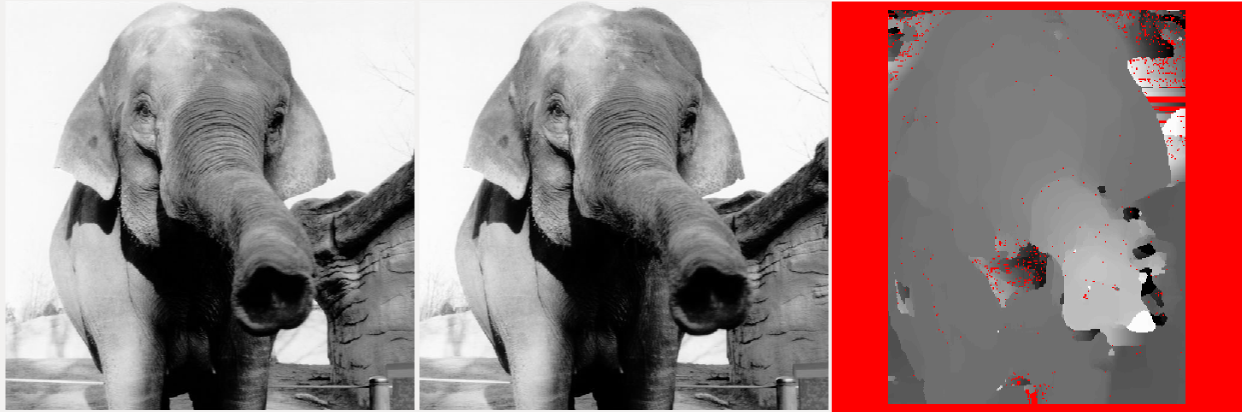
\includegraphics[width=0.6\linewidth]{images/elefant.png}
\caption{Testbilder Elefant: links, rechts und Ergebnis}%
\label{fig:elefant}
\end{figure}
Gemessen wurde die Zeit, die von der jeweiligen Implementierung für das Testbild gebraucht wurde. Für mehr Testdaten wurde die Auflösung des Bildes mehrfach in 10\% Schritten reduziert.\\

\begin{figure}[H]
\begin{tikzpicture}
\begin{axis}[
	scale only axis, % The height and width argument only apply to the actual axis
    height=6.9cm,
    width=.9\textwidth,
    xlabel={Auflösung (\%)},
    ylabel={Laufzeit (ms)},
    xmin=0, xmax=100,
    ymin=0, ymax=20000,
    %xmin=10, xmax=20,
    %ymin=0, ymax=300,
    xtick={0,20,40,60,80,100},
    ytick={0, 4000, 8000, 12000, 16000, 20000},
    legend pos=north west,
    ymajorgrids=true,
    grid style=dashed,
]
 
\addplot[
    color=blue,
    mark=square,
    ]
    coordinates {
    (10,0)
    (20,258)
    (30,975)
    (40,2080)
    (50,3593)
    (60,7471)
    (70,8470)
    (80,9945)
    (90,14976)
    (100,19699)
    };
    \addlegendentry{Java (Singlethreaded)}
    
\addplot[
    color=green,
    mark=square,
    ]
    coordinates {
    (10,2)
    (20,97)
    (30,363)
    (40,601)
    (50,986)
    (60,1530)
    (70,2136)
    (80,2754)
    (90,3472)
    (100,4559)
    };
    \addlegendentry{Java (Executor)}
    
\addplot[
    color=red,
    mark=square,
    ]
    coordinates {
    (10,2)
    (20,87)
    (30,311)
    (40,577)
    (50,747)
    (60,1362)
    (70,1792)
    (80,2370)
    (90,3493)
    (100,4857)
    };
    \addlegendentry{Java (Bildabschnitte)}   
    
\addplot[
    color=magenta,
    mark=square,
    ]
    coordinates {
    (10,0)
    (20,50)
    (30,167)
    (40,242)
    (50,458)
    (60,669)
    (70,917)
    (80,1200)
    (90,1543)
    (100,1882)
    };
    \addlegendentry{C (Bildabschnitte)}
    
\addplot[
    color=cyan,
    mark=square,
    ]
    coordinates {
    (10,30)
    (20,40)
    (30,60)
    (40,82)
    (50,93)
    (60,126)
    (70,173)
    (80,219)
    (90,283)
    (100,346)
    };
    \addlegendentry{CUDA}
 
\end{axis}
\end{tikzpicture}
\linespread{.3}\selectfont{}
\caption{Graph mit Laufzeiten der Implementierungsvarianten}
\end{figure}

Bei 10\% Auflösung ($69\times69$) ist CUDA die langsamste Lösung, doch schon bei 20\% Auflösung \sloppy ($138\times138$)
ist CUDA schneller als alle anderen Varianten und die Differenz wächst je höher die Auflösung wird.\\
\\
Die Java Single-Core Lösung ist wie vorhergesagt die langsamste Implementierung. Die Ausnahme ist bei 10\% Auflösung wo
sie die schnellste ist. \\
\\
Die beiden Java Multicore Implementierungen liefern nahezu identische Messergebnisse, wobei die Executor Variante
geringere Schwankungen beim Messen aufwies. Performance-technisch scheint es kaum einen Unterschied zu machen ob das
Bild in Abschnitte aufgeteilt wird oder Pixel für Pixel von Threads abgearbeitet wird.\\
\\
Vergleicht man die Ergebnisse von der Bildabschnitts-Aufteilung in Java und C wird deutlich, dass die C-Variante
schneller ist und kaum schwankt während die bereits erwähnten Schwankungen in der Java Implementierung durchaus merkbar
waren. Das JNI Interface kopiert die Bilddaten in den Speicher des C Programms und zurück nach Java. Da dies nur am
Anfang bzw. Ende des C-Programms passiert ist der Overhead gering.\\
\\
Die Messergebnisse zeigen dass CUDA definitiv zu bevorzugen ist, sofern es vorhanden ist. Nur bei sehr kleinen Bildern
sind andere Ansätze ähnlich schnell, doch je größer die Bilder werden desto schneller ist CUDA. Zwingend benötigt ist
es jedoch nicht. Auch wenn die Zeiten von Multicore-Prozessor-Lösungen deutlich höher sind als bei CUDA, können sie
Ergebnisse in tolerierbaren Zeiten berechnen, sofern die Bildgrößen in einem bestimmten Rahmen bleiben.
  
\section{Zusammenfassung}
% Nennen der wesentlichen Methoden und Resultate. Kurze, ehrliche Bewertung.
Die Evaluation der Messergebnisse veranschaulicht sehr gut, dass Nebenläufigkeit bei der Berechnung von
Tiefeinformationen aus stereoskopischen Bildern den größten Einfluss hat, welche Strategie genau verwendet wird ist
weniger wichtig für die Performance, kann sich aber in der Vorhersagbarkeit der Laufzeit niederschlagen, wie die
Messdaten der Java Programme darlegen. \\
Die Programmiersprache hingegen hat Einfluss auf die Performance, wobei
Ahead-of-time Kompilierung einen Performancegewinn bringt. Der Overhead des JNI Interface ist hierbei zu
vernachlässigen da nur wenige Funktionen über das Interface aufgerufen werden.
%\begin{itemize}
%  \item Nebenläufigkeit wichtig
%  \item Genaue Strategie eher unwichtig.
%  \item C schneller als java, dafür aber Aufwand für native calls
%  \item Overhead zu vernachlässigen 
%\end{itemize}

\section{Ausblick}
% Welche Fragen sind noch offen? Welche davon sollen in der eigenen Gruppe bearbeitet werden?
Damit die Ergebnisse dieser Arbeit in einer reale Umgebung überprüft werden können, wäre es möglich eine
Smartphone App zu entwickeln. Diese sollte die Aufnahme eines Bilderpaares und die anschließende Ermittlung der
Tiefeninformationen mittels Disparitätenberechnung erlauben. \\
Die Implementierung könnte in Java und, z.B. mittels des Android Native Development Kit (NDK), in C++ geschehen.
Es gibt sogar bereits einige Geräte (z.b. mit dem Nvidia Tegra Ein-Chip-System), die CUDA unterstützen \cite{codeworks}.
Mit diesen könnte überprüft werden, ob der immense Leistungsvorsprung von CUDA auch auf mobilen Geräten vorhanden ist. 


%\printbibliography
%\bibliographystyle{babplain}%
\bibliographystyle{babunsrt}%
\bibliography{quellen}% 

% \textcolor{tubsSecondary}{Dies ist ein Text in \texttt{tubsSecondary}.} \\ 
% \textcolor{tubsViolet}{Dies ist ein Text in \texttt{tubsViolet}.} \\
% \textcolor{tubsGreenDark}{Dies ist ein Text in \texttt{tubsGreenDark}.} \\
% 
% Siehe \autoref{fig:testbild}.
% \begin{figure}[htp]
% \begin{center}
%   
\includegraphics[width=.7\textwidth]{images/ibr}
%   \caption[Test Bild]{Test Bild}
%   \label{fig:testbild}
% \end{center}
% \end{figure}

\end{document}